\subsection{Detalls d'implementació}

    \paragraph{}
    Abans de destacar els detalls d'implementació d'aquesta funcionalitat i de forma anàloga a les dues funcionalitats anteriors, comentar, que només el controlador que gestiona aquesta funcionalitat, està format per tres-centes línies de codi i en conseqüència, manca de sentit intentar representar totes les funcionalitats i aspectes d'aquest en la memòria. Per tant, tot el codi que es trobarà en els següents apartats, ha estat simplificat per facilitar-ne la comprensió.

    El controlador encarregat del funcionament de l'evolució temporal d'esdeveniments és el fitxer \emph{facts.js}.

    \subsubsection{Validació del formulari de cerca}

\paragraph{}
A diferència de la funcionalitat de cerca general, aquesta funcionalitat sí que realitza una validació més exhaustiva dels valors introduïts per l'usuari, ja que una configuració incorrecta d'aquests, resultaria en l’obtenció de zero resultats.

Han estat implementades dues menes de validacions diferents. La coneguda com a validació en línia i la validació del formulari quan es prem el botó de cerca.

La validació en línia, s'activa quan l'usuari surt d'un camp del formulari i s'aprofita aquest moment, per mostrar el marc del camp en vermell, si aquest conté algun error o en verd, si el valor introduït és correcte. L'objectiu d'aquesta validació és facilitar a l'usuari la comprensió dels errors i corregir-los al més aviat possible; reduint així, la frustració en el moment de realitzar la cerca.

Per activar la validació en línia, s'utilitza la funció de jQuery \emph{onFocusOut()}, en conjunció a les classes de Bootstrap \emph{has-success} o \emph{has-error}. Aquestes classes, pinten la bora dels camps del formulari de color verd o vermell, de forma respectiva.

\begin{lstlisting}[style=rawOwn,caption={Activació de la validació en línia}]
$(`.form-vali').focusout(function() {
    if(inlineValidation($(this).attr(`id'))) {
        $(this).parent().removeClass(`has-success');
        $(this).parent().addClass(`has-error');
    }
    else {
        $(this).parent().removeClass(`has-error');
        $(this).parent().addClass(`has-success');
    }
});
\end{lstlisting}

Com es pot observar en el bloc de codi anterior, per tal de comprovar si un camp és vàlid o no, es crida a la funció \emph{inlineValidation(param)}, amb l’identificador del camp a comprovar. Aquesta funció és reutilitzada tant per la validació en línia, com per la validació en el moment de cerca.

Les regles de validació per cada un dels camps del formulari, s'especifiquen a continuació:

\begin{itemize}
    \item \textbf{Cognom:} Si el paràmetre té longitud zero, es mostra un error.
    \item \textbf{Països:} Si no s'ha seleccionat com a mínim un país, es mostra un error.
    \item \textbf{Any de naixement:} Si la longitud és diferent de quatre o no és un número, es mostra un error.
    \item \textbf{Rang:} Si el camp no està buit i la longitud és diferent de quatre o no és un número, es mostra un error.
    \item \textbf{Interval:} Si els paràmetres \emph{any de naixement} i \emph{rang} són diferents, el paràmetre \emph{rang} no és buit i \emph{l’interval} no està especificat o no és un nombre, es mostra un error.
\end{itemize}

La imatge~\ref{fig:surnamesError}, mostra a la vegada la validació en línia (marc dels camps del formulari en vermell o verd) i la caixa d'errors, que informa l'usuari dels errors produïts de forma més detallada, quan prem el botó de buscar amb paràmetres incorrectes.

\begin{figure}[h]
    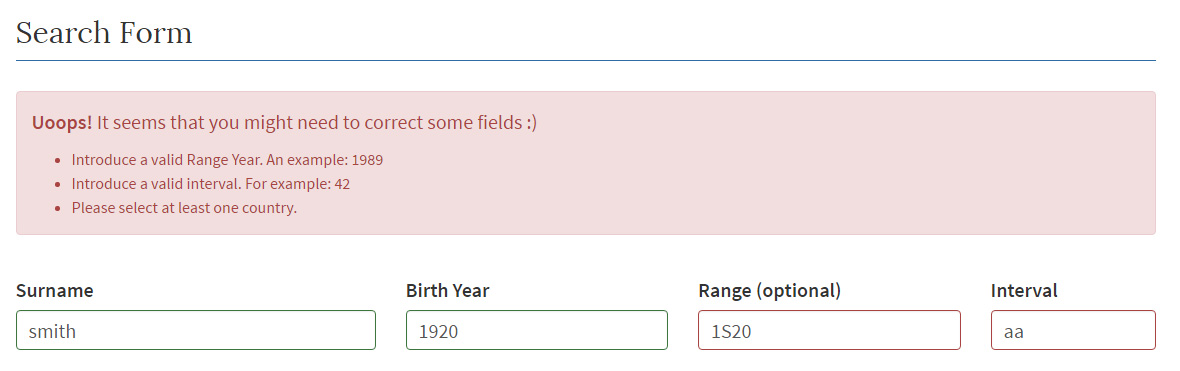
\includegraphics[width=\linewidth]{11/03_surnamesSearch/01_formValidation}
    \centering
    \caption{Exemples d'error en els formularis decerca}\label{fig:surnamesError}
\end{figure}

Si totes les validacions són superades, quan el formulari és enviat cap al SDK, s'escapen els paràmetres llegits de la mateixa forma que s'ha explicat per la funcionalitat de cerca en l’arbre familiar.

    \subsubsection{Regulació de les crides asíncrones}

\paragraph{}
De la mateixa forma que la funcionalitat expansió geogràfica d’un cognom, aquesta funcionalitat llança múltiples crides asíncrones contra el SDK de FamilySearch.

En concret, aquesta funcionalitat, sempre llença onze crides que per evitar ser bloquejades per la funcionalitat de `throttling' de l’API de FamilySearch, han estat serialitzades imposant una pausa de dos segons i mig entre crida i crida.

Aquesta serialització s'ha aconseguit, de forma anàloga a la descrita en detall a la funcionalitat anterior, mitjançant la funció \emph{setTimeout()} de jQuery i el paràmetre \emph{apiDELAY}, que s'encarrega d'indicar l'interval d'espera entre les diferents crides. També s'han encapsulat les crides en una funció, que emmagatzema com a paràmetre a quina de les onze crides correspon la iteració.

A continuació, mostrem el bloc de codi reduït, que representa la serialització de les crides a l’API.

\begin{lstlisting}[style=rawOwn,caption={Separació manual de les crides asíncrones al SDK}]
for(var i = 0; i < 11; i++) {
    ...
    (function(i) {
        setTimeout(function() {
            ...
            client.getPersonSearch(params).then(function(searchResponse) {
            var total = searchResponse.getResultsCount();
            linechartRows[i].push(String(firstYear+i));
            linechartRows[i].push(total);
            ...
            });
        }, apiDELAY*i);
    }(i));
}
\end{lstlisting}

Aquestes crides retornen al controlador una per una i encara que no podem garantir l'ordre de rebuda, s’espera que en la gran majoria dels casos, aquest es correspongui a l’ordre d’enviament. De totes maneres, gràcies al paràmetre \emph{i}, empaquetat en cada una de les crides, podem emmagatzemar les dades retornades pel SDK al lloc que els hi correspon de la matriu \emph{linechartRows}.

La variable global encarregada de guardar els resultats de les diferents crides al SDK és la mateixa que la utilitzada pel gràfic de línies de la funcionalitat expansió geogràfica d'un cognom, però que en aquest cas, consisteix en una matriu d'una sola columna, on la columna representa la localització cercada i cada fila, el valor per un any concret.

Explicar que utilitzem una matriu d'una sola columna, en comptes d'un vector, perquè aquest és el format que espera l'API de Google, si volem que el gràfic representi la quantitat d'instàncies trobades en l'eix vertical i els anys a l'eix horitzontal.

La línia de codi responsable de guardar els valors per cada crida a l’API, ha estat mostrada en el bloc de codi anterior i en concret, a les files vuit i nou. Recordem, que el paràmetre \emph{i} fa referència a la iteració del bucle executada i per extensió, a quin any fan referència les dades respecta els onze anys de l’interval cercat.

    \subsubsection{Impressió dels gràfics}

\paragraph{}
A causa del funcionament de la funcionalitat, resulta fàcil, que a la mínima que es realitza una cerca mitjanment gran, aquesta tardi més d'un minut en completar-se.

Per tal de transmetre sensació de moviment i que el sistema està treballant, hem introduït a la funcionalitat la capacitat d'anar pintant els gràfics de cada any de l'interval, a mesura que les dades van quedant disponibles. És a dir, que no cal esperar fins al final de la cerca, per poder començar a explorar els resultats.

Per aconseguir aquest efecte, disposem de variables globals que comptabilitzen el nombre de cerques que ja han retornat del SDK i cada cop que les dades d'un any queden completades, es pinta el mapa geogràfic i el gràfic de barres, relatiu a l'any. Un cop es completen les dades de tots els anys, es pinta el gràfic de línies.

Els gràfics es pinten mitjançant la crida a l'API de GoogleCharts. Per pintar qualsevol gràfic, sempre se segueix un procés similar:

\begin{enumerate}
    \item Transformació de les dades a un format que Google utilitzarà després per crear el gràfic.
    \item Creació del tipus de gràfic desitjat, mitjançant una crida a l'API de Google i selecció del contenidor HTML en el qual volem inserir el gràfic.
    \item Renderització del gràfic en el HTML.
\end{enumerate}

Pel mapa geogràfic, gràcies a la forma en què s’han anat emmagatzemant les dades, el procés és relativament simple. Recordem, que cada fila de la matriu \emph{geomap\-Countries} representa els valors d’un any i cada columna, un país diferent.

\begin{lstlisting}[style=rawOwn,caption={Creació del mapa geogràfic}]
function printGeomap(i) {
    var geomapData = google.visualization.arrayToDataTable(geomapCountries[i]);
    geomap = new google.visualization.GeoChart(document.getElementById(`geomap'));
    geomap.draw(geomapData, geomapOptions);
}
\end{lstlisting}

Per pintar el gràfic de barres, el procés és molt similar al del mapa geogràfic, però primer realitzem un petit tractament de les dades, per tal d'ordenar els països de més a menys instàncies trobades i obtenir així, una representació més clara de la resposta.

Per aconseguir-ho, es crea una funció de comparació dedicada (\emph{compare\-Countries}), que compararà els diferents elements de l'objecte \emph{barchartCountries}, a través de la funció \emph{sort}, pròpia de Javascript.

\begin{lstlisting}[style=rawOwn,caption={Creació del gràfic de barres}]
function compareCountries(a, b) {
    if(parseInt(a[1]) < parseInt(b[1])) return 1;
    else if(parseInt(a[1]) > parseInt(b[1])) return -1;
    else return 0;
}

function printBarchart(i) {
    // Sort data
    var barchartCountries = geomapCountries[i];
    var first = barchartCountries.splice(0, 1);
    barchartCountries.sort(compareCountries);
    barchartCountries.unshift(first[0]);

    // transform and plot
    var barchartData = google.visualization.arrayToDataTable(barchartCountries);
    barchart = new google.charts.Bar(document.getElementById(`barchart'));
    barchart.draw(barchartData, barchartOptions);
}
\end{lstlisting}

En últim lloc, el gràfic de línies també resulta bastant fàcil de pintar, ja que gràcies a la forma en què s’han emmagatzemat les dades, no fa falta realitzar cap tractament especial sobre aquestes, abans de pintar-les.

\begin{lstlisting}[style=rawOwn,caption={Creació del gràfic de línies}]
function printLinechart() {
    ...
    linechartData.addRows(linechartRows);
    linechart = new google.charts.Line(document.getElementById(`linechart'));
    linechart.draw(linechartData, linechartOptions);
    ...
}
\end{lstlisting}

Les figures~\ref{fig:geomap}, \ref{fig:barchart} i \ref{fig:linechart}, ofereixen una visualització dels diferents gràfics disponibles.

\begin{figure}[h]
    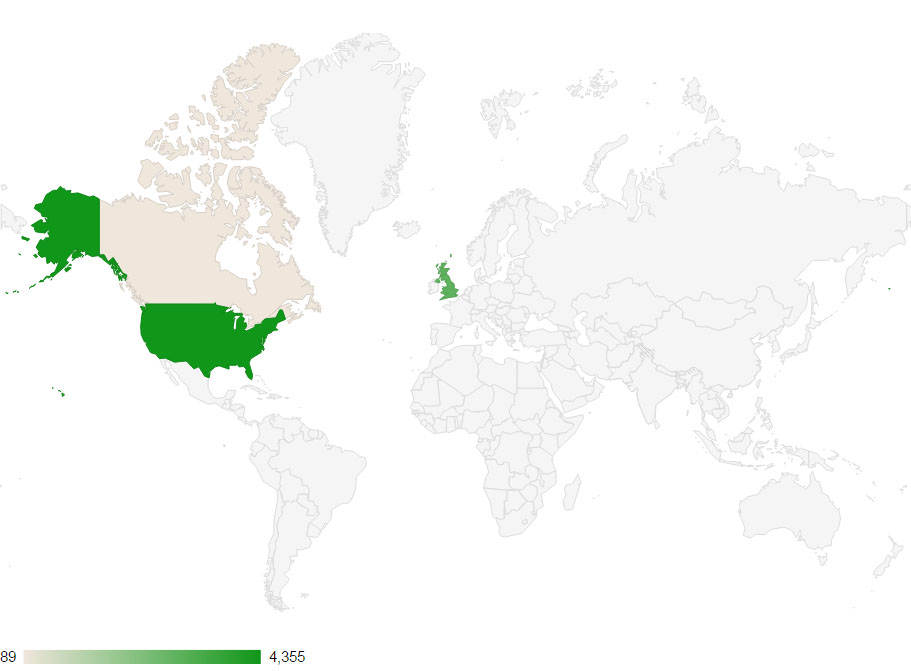
\includegraphics[width=\linewidth]{11/03_surnamesSearch/02_geomapDesktop2}
    \centering
    \caption{Mapa geogràfic}\label{fig:geomap}
\end{figure}

\begin{figure}[h]
    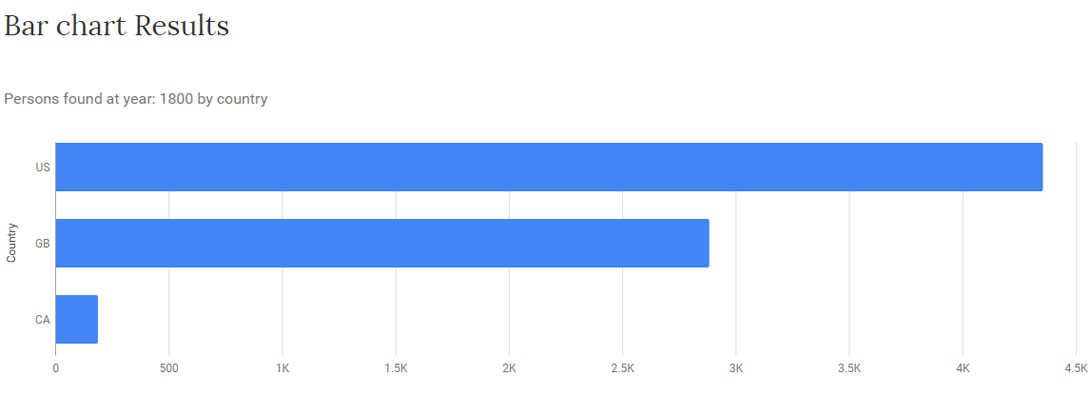
\includegraphics[width=\linewidth]{11/03_surnamesSearch/03_barChartDesktop2}
    \centering
    \caption{Gràfic de barres}\label{fig:barchart}
\end{figure}

\begin{figure}[h]
    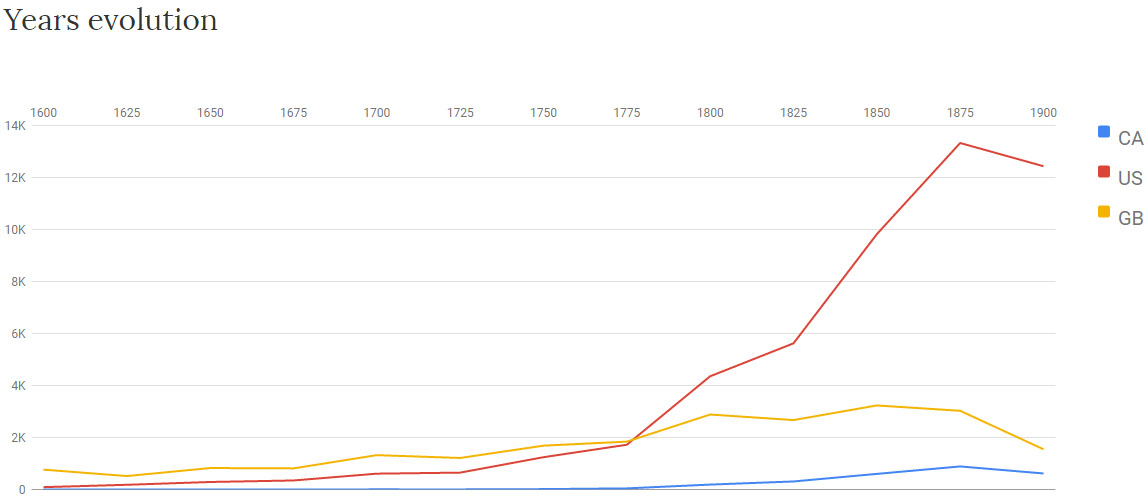
\includegraphics[width=\linewidth]{11/03_surnamesSearch/04_yearsEvolutionDesktop3}
    \centering
    \caption{Gràfic de línies}\label{fig:linechart}
\end{figure}

